\documentclass[12pt,a4paper]{article}
\usepackage[utf8]{inputenc}
\usepackage[T1]{fontenc}
\usepackage{amsmath}
\usepackage{amsfonts}
\usepackage{amssymb}
\usepackage{lipsum}
\usepackage{textcomp}

\usepackage{makecell} % linebreak dans une cellule
\usepackage{multicol} % twocols localement
\usepackage{vwcol} % idem mais avec largeur variable
\usepackage{color, colortbl} % colorer les tableaux
\usepackage{enumitem} % utiliser des lettres pour énumérer
\usepackage{wrapfig} % insérer des images dans dutexte
\usepackage{dashundergaps} % transformer du texte en ________
\usepackage{MnSymbol,wasysym} % smileys
\usepackage{ifthen}
\usepackage{soul} % teste barré \st

% --- geometry ---
\usepackage{geometry}
\geometry{legalpaper, margin=2cm}
% ---

% --- xcolor ---
\usepackage{xcolor}
\definecolor{lightgray}{gray}{0.9}
% ---

% --- tcolorboxes ---
\usepackage[most]{tcolorbox}
\newtcolorbox{definition}[2][]{%
  attach boxed title to top left
               = {yshift=-8pt},
  colback      = white,
  colframe     = gray,
  fonttitle    = \bfseries,
  colbacktitle = gray,
  title        = #2,#1,
  enhanced,
}
% ---


\renewcommand{\baselinestretch}{1.15} % augmenter l'interligne

\dashundergapssetup{
	teacher-gap-format=underline,
	gap-widen
}



\author{Paul Clavier}
\title{Chapitre 7 - Cercles et polygones réguliers}

\begin{document}

% --- Section & subsection renum ---
\renewcommand\thesection{\Roman{section}}
\renewcommand\thesubsection{\arabic{subsection}}
% ---

% --- Selection manuelle de la version ---
%\def\isprof{true}
% ---

% --- Selection automatique de la version ---
\ifdefined\isprof
	\TeacherModeOn
\fi

% ---



\begin{center}
	\fbox{\parbox{\dimexpr\linewidth-2\fboxsep-2\fboxrule\relax}{\centering\huge Chapitre 7 - Cercles et polygones réguliers}}
\end{center}

\section{Le Cercle}
\begin{definition}{Définition}
Un cercle de centre O est l'ensemble des points situés à une même distance du point O. Cette distance est appelée le rayon du cercle.
\end{definition}

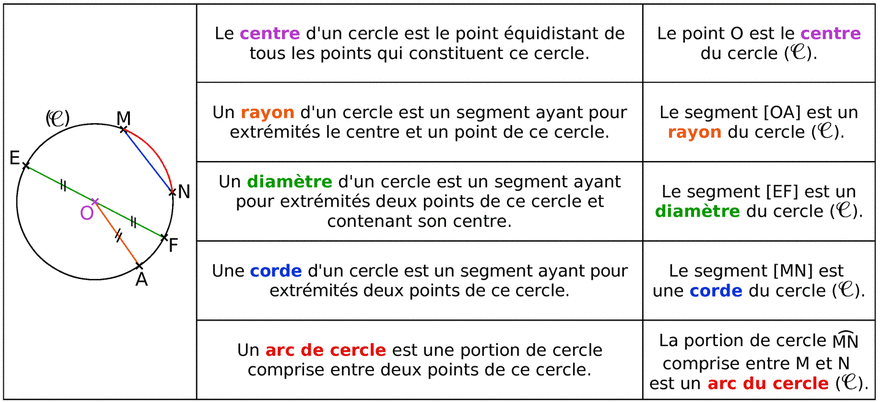
\includegraphics[scale=0.54]{img/Cercle.png} 

\section{Les triangles}

\begin{minipage}{0.5\textwidth}
\begin{definition}{Définition}
Un triangle est un polygone à trois cotés.
\end{definition}
\end{minipage}
\begin{minipage}{0.5\textwidth}
\begin{definition}{Vocabulaire}
Un triangle a trois sommets et trois cotés.
\end{definition}
\end{minipage}

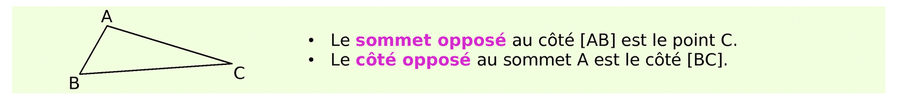
\includegraphics[scale=0.72]{img/triangle-exemple.png} 

\subsection{Les triangles rectangles}

\begin{minipage}{0.5\textwidth}
\begin{definition}{Définition}
Un triangle rectangle est un triangle qui a un angle droit.
\end{definition}
\end{minipage}
\begin{minipage}{0.5\textwidth}
\begin{definition}{Vocabulaire}
Le coté opposé à l'angle droit est appelé l'hypoténuse.
\end{definition}
\end{minipage}

\subsection{Les triangles isocèles}

\begin{minipage}{0.5\textwidth}
\begin{definition}{Définition}
Un triangle isocèle est un triangle qui a deux cotés de même longueur.
\end{definition}
\end{minipage}
\begin{minipage}{0.5\textwidth}
\begin{definition}{Vocabulaire}
\begin{itemize}
\item Le sommet commun 	aux cotés de même longueur est appelé le sommet principal.
\item Le coté opposé au sommet principal est appelé la base.
\end{itemize}
\end{definition}
\end{minipage}
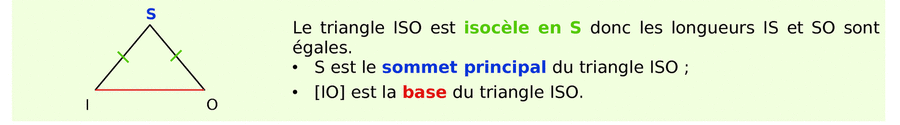
\includegraphics[scale=0.56]{img/triangle-exemple2.png} 
\subsection{Les triangles équilatéraux}

\begin{definition}{Définition}
Un triangle équilatéral est un triangle qui à ses trois cotés de même longueur.
\end{definition}

\section{Les Quadrilatères}
\begin{minipage}{0.5\textwidth}
\begin{definition}{Définition}
Un quadrilatère est un polygone à quatre cotés.
\end{definition}
\end{minipage}
\begin{minipage}{0.5\textwidth}
\begin{definition}{Vocabulaire}
Un quadrilatère à quatre sommets, quatre cotés et deux diagonales.
\end{definition}
\end{minipage}
\subsection{Le rectangle}
\begin{definition}{Vocabulaire}
Un rectangle est un quadrilatère qui a ses quatre angles droits.
\end{definition}
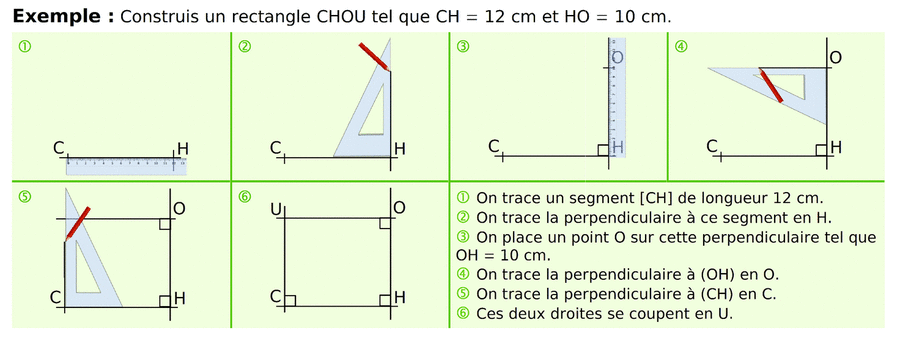
\includegraphics[scale=0.5]{img/rectangle.png} 
\begin{definition}{Propriété}
Dans un rectangle, les cotés opposés sont de même longueur.
\end{definition}

\subsection{Le losange}
\begin{minipage}{0,7\textwidth}
\begin{definition}{Définition}
Un losange est un quadrilatère qui a ses quatre cotés de même longueur.
\end{definition}
\end{minipage}
\begin{minipage}{0,3\textwidth}
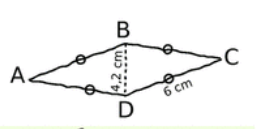
\includegraphics[scale=0.5]{img/losange.png} 
\end{minipage}

\subsection{Le carré}
\begin{definition}{Définition}
Un carré est un quadrilatère qui a ses quatre cotés de même longueur et ses quatre angles droits.
\end{definition}
\begin{definition}{Remarque}
Un carré est à la fois un losange et un rectangle.
\end{definition}

\subsection{Le parallélogramme}
\begin{definition}{Définition}
Un parallélogramme est un quadrilatère qui a ses cotés opposés parallèles.
\end{definition}

\end{document}